%%%%%%%%%%%%%%%%%%%%%%%%%%%%%%%%%%%%%%%%%%%%%%%%%%%%%%%%%%%%%%%%%%%%%%%%
%    INSTITUTE OF PHYSICS PUBLISHING                                   %
%                                                                      %
%   `Preparing an article for publication in an Institute of Physics   %
%    Publishing journal using LaTeX'                                   %
%                                                                      %
%    LaTeX source code `ioplau2e.tex' used to generate `author         %
%    guidelines', the documentation explaining and demonstrating use   %
%    of the Institute of Physics Publishing LaTeX preprint files       %
%    `iopart.cls, iopart12.clo and iopart10.clo'.                      %
%                                                                      %
%    `ioplau2e.tex' itself uses LaTeX with `iopart.cls'                %
%                                                                      %
%%%%%%%%%%%%%%%%%%%%%%%%%%%%%%%%%%
%
%
% First we have a character check
%
% ! exclamation mark    " double quote  
% # hash                ` opening quote (grave)
% & ampersand           ' closing quote (acute)
% $ dollar              % percent       
% ( open parenthesis    ) close paren.  
% - hyphen              = equals sign
% | vertical bar        ~ tilde         
% @ at sign             _ underscore
% { open curly brace    } close curly   
% [ open square         ] close square bracket
% + plus sign           ; semi-colon    
% * asterisk            : colon
% < open angle bracket  > close angle   
% , comma               . full stop
% ? question mark       / forward slash 
% \ backslash           ^ circumflex
%
% ABCDEFGHIJKLMNOPQRSTUVWXYZ 
% abcdefghijklmnopqrstuvwxyz 
% 1234567890
%
%%%%%%%%%%%%%%%%%%%%%%%%%%%%%%%%%%%%%%%%%%%%%%%%%%%%%%%%%%%%%%%%%%%
%
\documentclass[12p]{iopart}
\newcommand{\gguide}{{\it Preparing graphics for IOP Publishing journals}}
%Uncomment next line if AMS fonts required
%\usepackage{iopams}  

\usepackage{graphicx}

\usepackage{hyperref}
\hypersetup{
	colorlinks=true,
	linkcolor=blue,
	filecolor=magenta,      
	urlcolor=cyan,
}

% bibliography
\usepackage[
	backend=biber,
	style=numeric,
	sorting=none
]{biblatex} 
\addbibresource{2021_WEST_ICRH_paper.bib}

% units
\usepackage{siunitx}

% alias
\newcommand{\ZT}{Z_{\mathrm{T}}}
\newcommand{\ZTSP}{Z_{\mathrm{T,SP}}}

\begin{document}

\title[WEST ICRH System Results]{WEST Actively Cooled Load Resilient Ion Cyclotron Resonance Heating System Results}

\author{J.Hillairet, P.Mollard, L.Colas, J.-M.Bernard, J.-M.Delaplanche, F.Durand, N.Faure, P.Garibaldi, G.Lombard, C.Bourdelle, C.Desgranges, E.Delmas, R.Dumont, A.Ekedahl, F.Ferlay, M.Goniche, C.Guillemaut, G.T.Hoang, P.Maget, R.Volpe and WEST Team}
\address{CEA, IRFM,	F-13108 St-Paul-Lez-Durance, France}

\author{W.Helou}
\address{Iter Organization
Route De Vinon-Sur-Verdon, Cs 90 046, 13067 St. Paul Lez Durance Cedex, France}

\author{G.Urbanczyk}
\address{Key Laboratory Of Optoelectronic Devices And Systems, College Of Physics And Optoelectronic Engineering
Shenzhen University, Shenzhen 518060, China}

\author{Y.Song, Q.Yang, Z.Chen, Y.Wang, H.Xu, S.Yuan, Y.Zhao}
\address{Institute Of Plasma Physics, Cas
Hefei, Anhui 230031, Pr China}

\author{F.Durodie, E.Lerche, R.Ragona}
\address{Laboratory For Plasma Physics, Royal Military Academy 
1000 Bruxelles, Belgium}

\author{N.Bertelli, M.Ono, S.Shiraiwa}
\address{Princeton Plasma Physics Laboratory
Princeton, Nj 08543, Usa}

\author{V.Bobkov}
\address{Max-Planck Institut Für Plasmaphysik
Boltzmannstraße 2, 85748 Garching, Germany}

\author{C.Klepper, C.Lau, E.Martin}
\address{Oak Ridge National Laboratory
1 Bethel Valley Rd, Oak Ridge, Tn 37830}

\author{B.Lu}
\address{Southwestern Institute Of Physics 
Po Box 432, Chengdu 610041, Pr China}

\author{R.Maggiora, D.Milanesio}
\address{Politecnico Di Torino, Department Of Electronics And Telecommunications}

\author{K.Vulliez}
\address{Cea, Liten 
F-38054 Grenoble, France}

\author{G.Wallace}
\address{Plasma Science And Fusion Center, Mit 
Cambridge, Ma, 02139, Usa}

\ead{julien.hillairets@cea.fr}
\vspace{10pt}

\begin{abstract}
Three identical new WEST Ion Cyclotron Resonance Heating (ICRH) antennas have been designed, assembled then commissioned on plasma from 2013 to 2019. The WEST ICRH system is both load-resilient and compatible with long-pulse operations. The three antennas have been successfully operated together on plasma in 2019 and 2020. The load resilience capability has been demonstrated and the antenna feedback controls for phase and matching have been developed. The breakdown detection systems have been validated and successfully protected the antennas. The use of ICRH in combination with Lower Hybrid has triggered the high confinement mode transitions identified on WEST.
\end{abstract}

%
% Uncomment for keywords
\vspace{2pc}
\noindent{\it Keywords}: ICRH, ICRF, WEST

% Uncomment for Submitted to journal title message
\submitto{\NF}
 
% For two-column output uncomment the next line and choose [10pt] rather than [12pt] in the \documentclass declaration
%\ioptwocol



\section{Introduction and antennas description}
One of the objectives of the WEST machine being to study high heat loads and particle fluxes in a fully metallic tokamak environment \cite{bucalossi2021, bourdelle2015}, the WEST external heating systems must be compatible with long-pulse ELMy H-mode and steady-state plasma operation. No Ion Cyclotron Resonance Heating (ICRH) system before ITER has had to deal with these two challenges simultaneously, i.e. ELMs resilience and Continuous Wave (CW) RF operation. To meet these objectives, three new identical ICRH antennas have been designed through a European collaboration and with CAS/ASIPP \cite{helou2015-1, hillairet2015-2, chen2015, vulliez2015}, within the framework of the Associated Laboratory IRFM-ASIPP \cite{yang2015}. The antennas have been manufactured at the Keye Company in Hefei under the supervision of ASIPP.

The three WEST ICRH antennas have been designed to satisfy the ICRH power requirements for WEST plasma scenarios, i.e. a total ICRH power up to \SI{9}{\mega\watt} (high power scenarios) or \SI{3}{\mega\watt} (high fluence scenarios) \cite{bourdelle2015}. RF frequency can be varied from 46 to \SI{65}{\mega\hertz} to fit the main WEST ICRH scheme, which consists of hydrogen-minority in deuterium plasmas. 

Each antenna is made of four short straps (2 toroidal $\times$ 2 poloidal) located in separated boxes behind a Faraday Screen (figure~\ref{fig:antenna}). The tilt angle of the Faraday Screen bars is close to the direction of the total magnetic field lines facing the antennas (\SI{7}{\degree}). Each toroidal side of an antenna is fed by a separate high power source. The phase between the left and right sides of each antenna is defined by the plasma control system, the default being dipole configuration. An FPGA-based PID controller modulates the right side generator source frequency (the left side being the reference) to maintain the requested phase with a response time of approximately \SI{50}{\micro\second}. Moreover, the frequencies at which antennas are operated are slightly shifted from the scenario request (around $\pm \SI{0.3}{\mega\hertz}$) to reduce cross-talk between antennas. All antennas are movable radially for optimizing the power coupling and thermal loads handling.

To cope with the fast changes of the electron density facing the antenna during ELMs, the antennas rely on internals conjugate-T \cite{bosia2003-1}: poloidal pairs of straps are connected to an adjustable series capacitor and fed from a common T-junction. Matching is achieving by tuning these capacitors such as the two parallel branches have complex conjugate admittances. If the impedance seen at the T-junction is in the range of 3 to \SI{6}{\ohm}, this feeding circuit allows maintaining the Standing Wave Ratio (SWR) below reasonable values for the generator (below $2{:}1$ for \SI{3}{\mega\watt} per antenna on WEST) within a large increase in antenna resistive loadings, such as the ones expected during ELMs. This load-tolerant electrical circuit has been successfully tested in few seconds pulses in Tore Supra \cite{vulliez2008} and JET \cite{durodie2012-1}. This choice was also motivated by the fact that no \SI{3}{\decibel} Continuous Wave (CW) couplers were available (and still) on the market and required important R\&D. The low impedance at the conjugate-T junction is then transformed to the feeding \SI{30}{\ohm} transmission lines by a fixed two-stage quarter-wave transformer.


\begin{figure}
	\centering
	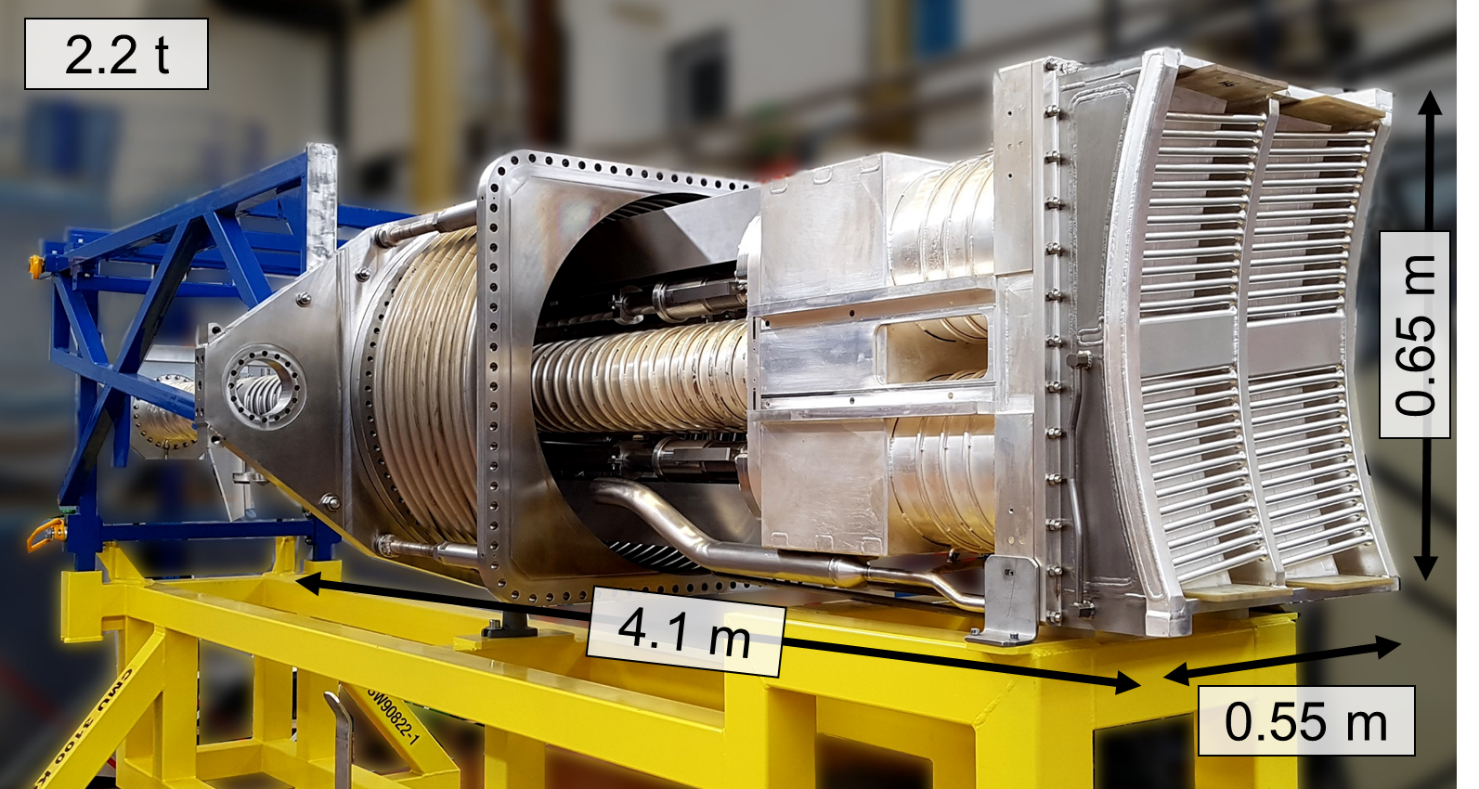
\includegraphics[width=0.95\linewidth]{figures/antenna}
	\caption{Picture of one WEST ICRH Antenna during its assembly and main dimensions.}
	\label{fig:antenna}
\end{figure}




Thanks to the collaboration between LPP-RMA and CEA, the experience gained with the JET ILA \cite{durodie2012-1} has been used during the WEST antenna design. In particular, the reliability of the operation of the capacitors has been improved with reduced mechanical stresses and the possibility to perform remote-diagnostic of the capacitor internal vacuum. Lessons were also learned from Tore Supra prototypes, to improve vacuum tightness and to bring water in all the parts of the antenna \cite{vulliez2008, vulliez2015}. The vacuum pumping of the impedance transformer sections has been improved and the pressure is monitored with two pressure gauges. Strap voltages are measured using D-dot electric field probes located between the capacitors and the straps (figure~\ref{fig:westicrhblockdiagram}). Strap currents are deduced analytically from these voltages, assuming the strap impedance is mostly reactive. Forward and reflected powers are measured by bi-directional couplers located at the rear of the antenna and at the generator plant. The forward RF power is feedback-controlled to keep voltages and currents below their maximum safety thresholds, set to \SI{28}{\kilo\volt} and \SI{915}{\ampere} respectively, with a fast response time of the order of \SI{10}{\micro\second} to avoid possible voltage or current overshoots during plasma disruptions.

\begin{figure}
	\centering
	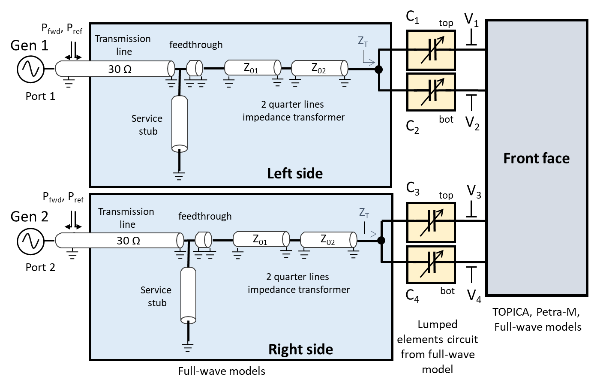
\includegraphics[width=0.95\linewidth]{figures/WEST_ICRH_block_diagram}
	\caption{Block diagram of a WEST ICRH antenna.}
	\label{fig:westicrhblockdiagram}
\end{figure}


A unique feature of these antennas is to satisfy the long pulse requirement of WEST. Antennas are fully water-cooled using two distinct water circuits: i) a high temperature/high pressure (up to \SI{200}{\celsius} during baking operation and \SI{70}{\celsius}/\SI{30}{\bar} bar during plasma operation) water circuit and ii) a low temperature/low pressure (\SI{25}{\celsius}/\SI{4}{\bar}) specifically designed to cool the antenna matching capacitors \cite{chen2015,vulliez2015}. However, some limitations remain in the thermal evolution of non-actively water-cooled components that could not be replaced or actively cooled, such as in the generator plant, transmission lines or vacuum feed-throughs. This implies a tuning of the total power as a function of the pulse duration, i.e. to \SI{9}{\mega\watt} /\SI{30}{\second}, \SI{6}{\mega\watt}/\SI{60}{\second} and \SI{3}{\mega\watt}/\SI{1000}{\second} \cite{hillairet2015-2}.

All antenna RF surfaces, such as the Faraday Screen, antenna box, straps, internal and external conductors, are silver-coated (\SI{10}{\micro\meter} Ni and around \SI{50}{\micro\meter} Ag, i.e. more than five times the skin depth). Lateral limiters are located on both sides of each antenna and protrude by \SI{2}{\centi\meter} from the edges of the Faraday Screen. These limiters are the ones used on Tore Supra and are made of CFC tiles coated with a double coating made of a first \SI{80}{\micro\meter} molybdenum layer followed by an \SI{80}{\micro\meter} tungsten (W) coating \cite{firdaouss2017-1, firdaouss2017}. While having high Z materials close to an ICRH antenna was known to increase the tungsten sputtering attributed to the acceleration of light impurity ions in the rectified RF sheaths \cite{bobkov2010}, this choice was motivated by the desire to keep a full W, reactor relevant machine \cite{bucalossi2014}.

An infrared thermography system monitors the antenna front-faces with a spatial resolution better than \SI{5}{\milli\metre}/pixel\cite{courtois2019}. Antenna limiters are protected with a real-time reduction of the RF power if the luminance temperature (i.e. with unity emissivity) exceeds a threshold initially determined either from material test bed or experience. The real-time protection of the ICRH antenna front-face is more challenging in WEST than in Tore-Supra\cite{colas2009}, in particular due to the low emissivity of their silver coating which reduces the surface temperature estimation accuracy \cite{aumeunier2021}. So far, the front-faces are monitored but without real-time feedback on RF power during plasma operations.

The WEST ICRH antenna design phase has been conducted from 2013 to 2014, followed by manufacturing in ASIPP from 2015 to 2017. Antenna elements were shipped to CEA, then silver coated and the antennas assembled in series from 2016 to 2019. The antennas have been commissioned on TITAN, then installed on WEST and operated progressively since 2018 \cite{bernard2017, bernard2019, helou2020}. In 2019, all three antennas were operated on WEST (figure~\ref{fig:ICRH_antenna_inside_WEST}). This paper reports the commissioning and the key results obtained on plasma with the full WEST ICRH system.

\begin{figure}
	\centering
	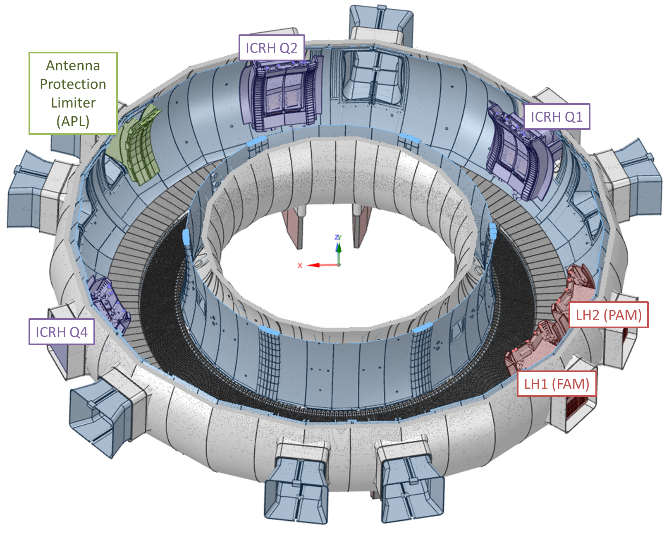
\includegraphics[width=0.95\linewidth]{figures/WEST_overview}
	\caption{WEST Top and 3D cut view. ICRH antennas are named after the equatorial port (Q) number they are inserted in: Q1, Q2 and Q4.}
	\label{fig:westoverview}
\end{figure}

\begin{figure}
	\centering
	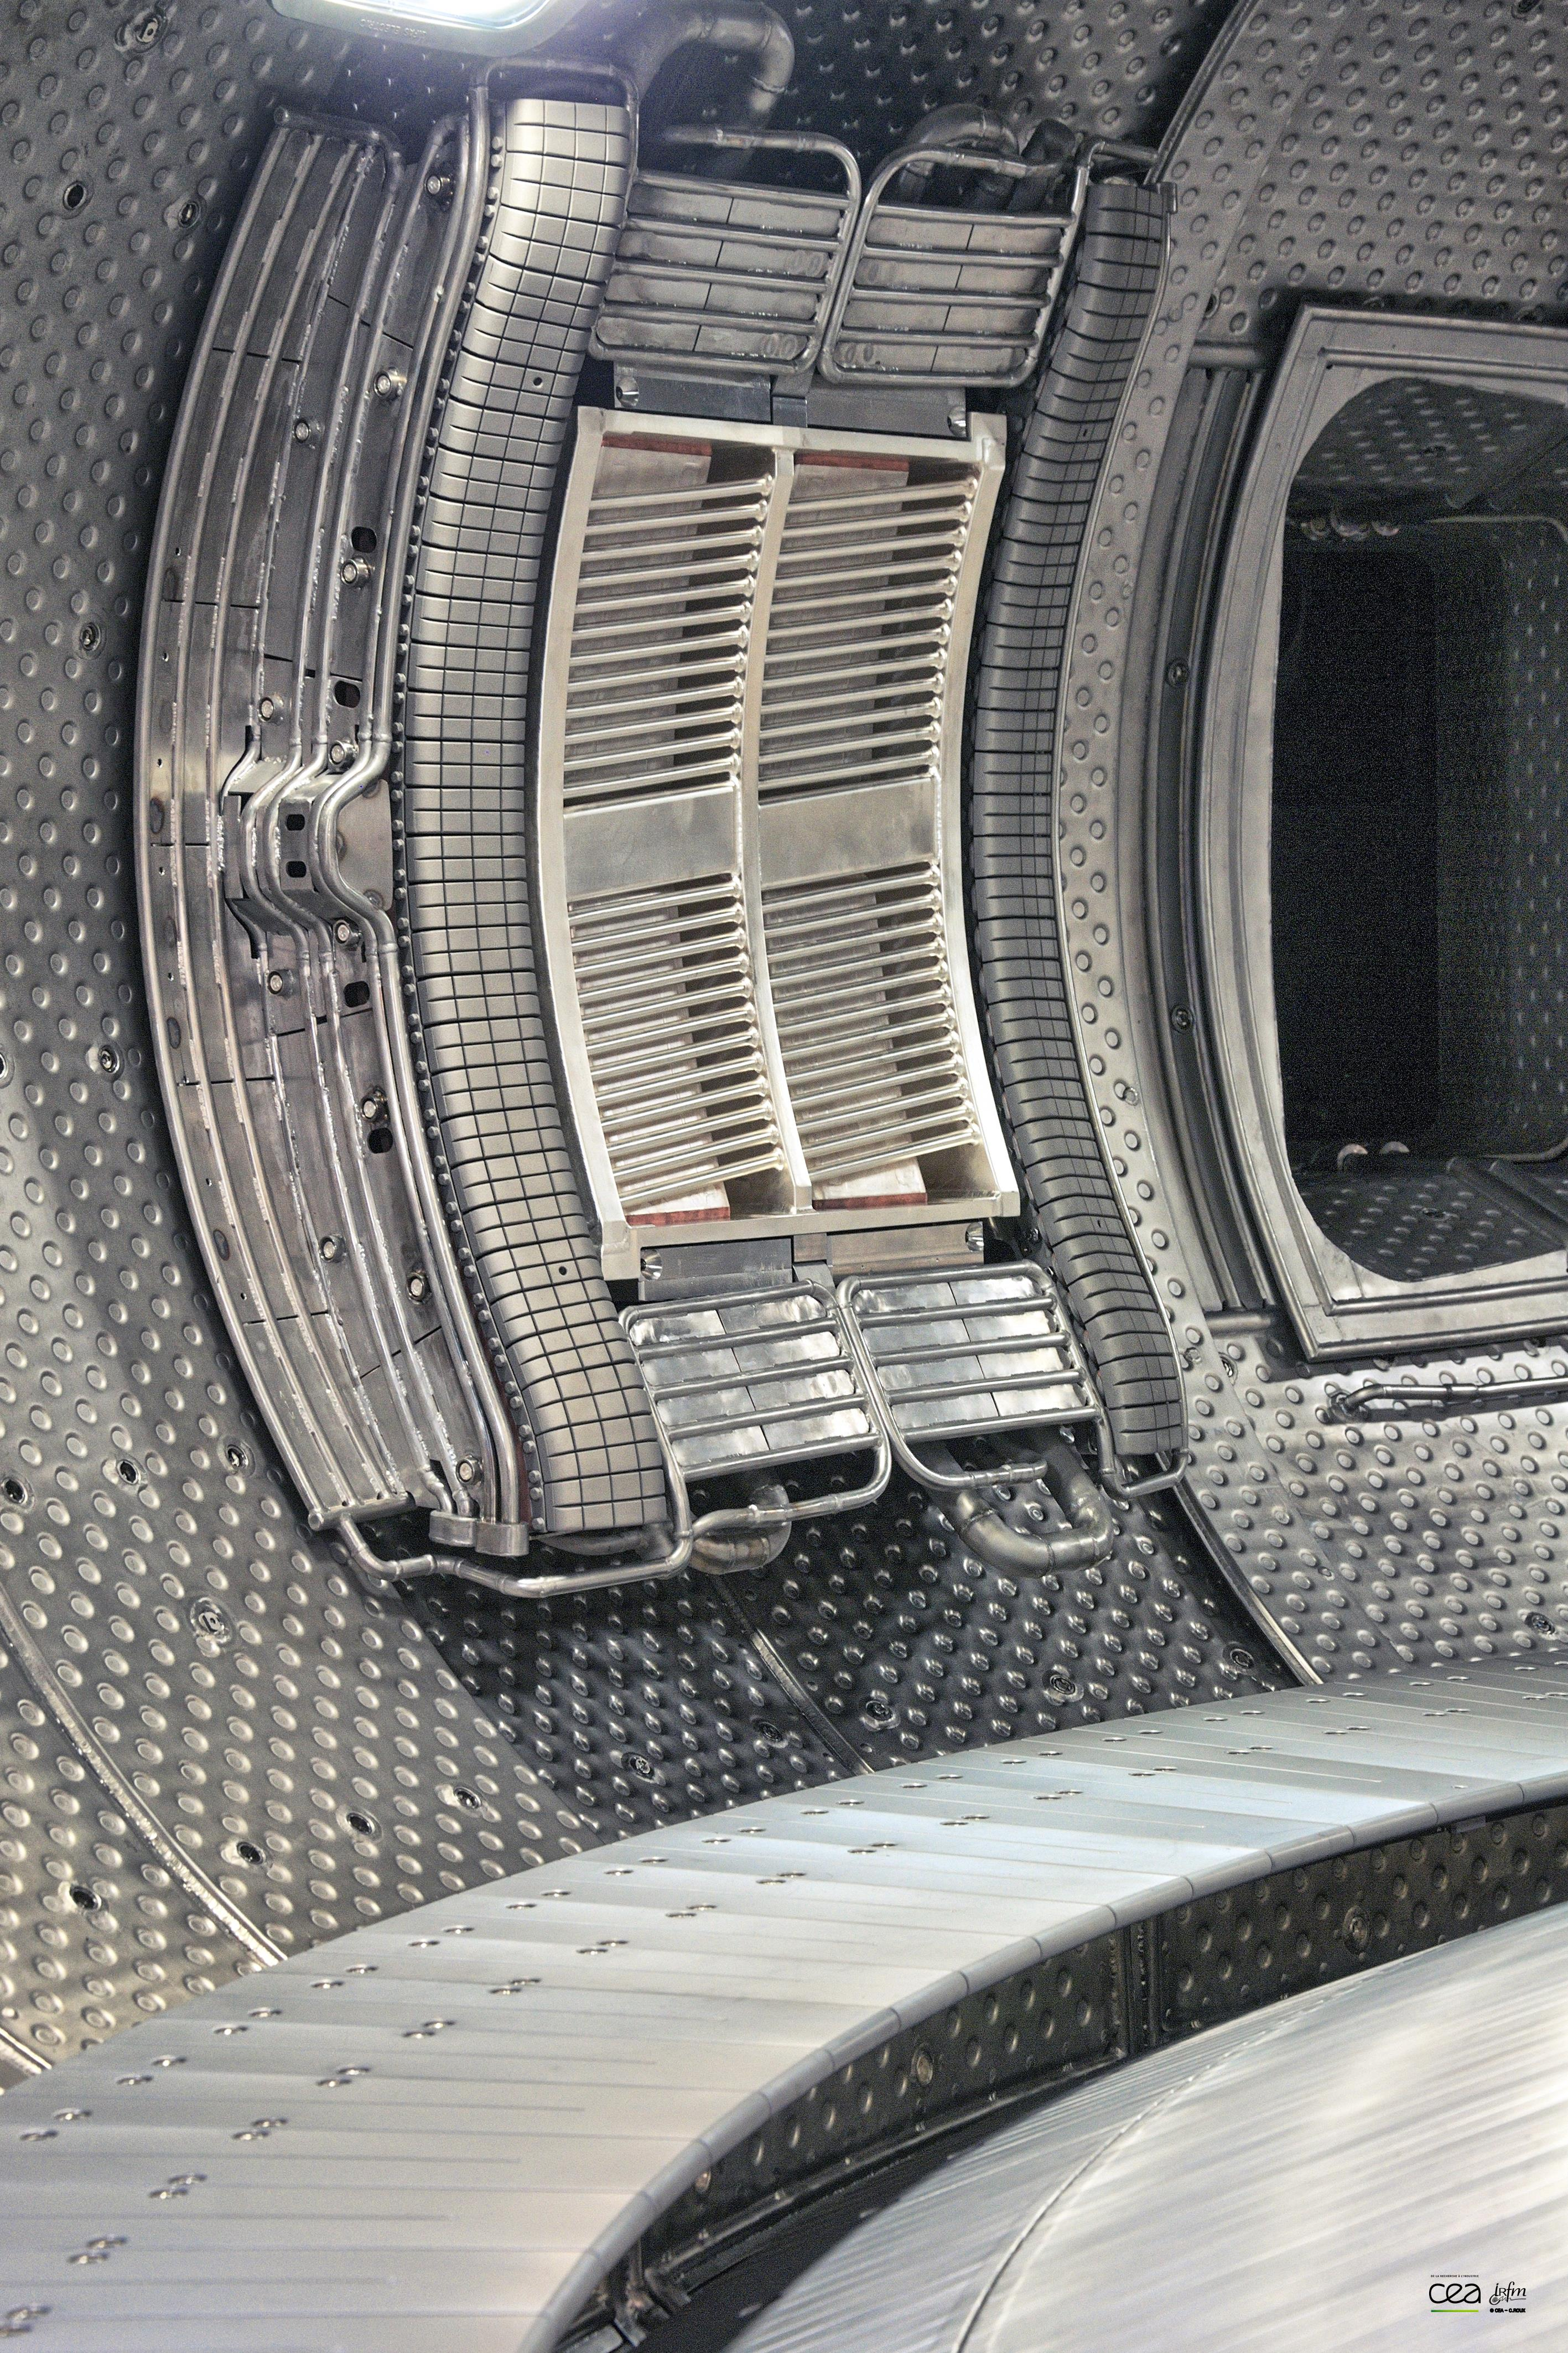
\includegraphics[width=0.7\linewidth]{figures/6}
	\caption{Picture of a WEST ICRH antenna inside the WEST machine, surrounded with its lateral W-coated limiters and steady-state heat flux shields @C.Roux}
	\label{fig:ICRH_antenna_inside_WEST}
\end{figure}


\section{RF Modelling}
The WEST ICRH RF modelling, described in more details in \cite{helou2015-2, hillairet2020-2}, is summarized in this section. The antenna RF model uses a combination of full-wave models of the antenna’s elements and equivalent lumped elements circuit of the tuning capacitors deduced from full-wave simulations (Figure 1). The evaluation of the scattering parameters of the 4-ports front-end facing the plasma computed using bespoke codes such as TOPICA \cite{milanesio2009} or Petra-M \cite{bertelli2020, shiraiwa2021}, or using commercial FEM software such as COMSOL in RAPLICASOL \cite{tierens2020-2}. The complete electrical circuit a WEST ICRH antenna is assembled using the open-source Python package scikit-rf\footnote{\url{http://scikit-rf.org}}  and can be found and used online\footnote{\url{https://github.com/jhillairet/WEST_IC_antenna}}. The overall model allows comparing voltages, currents, powers and phases to measurements as illustrated in Section 4 and can be used in the control room to assist ICRH operators in antenna tuning. Future work will focus on making “digital twins” of each antenna, enabling operators to interpret the antenna measured responses (post-pulse) and to guide operators in optimizing the antennas for the next plasma pulse.

\section{Antennas Commissioning}
\subsection{Low power RF tests}
During the antenna assembly, calibrations have been performed of components not accessible in later stages, such as voltage probes and vacuum RF cables. Once done, cold RF tests were performed to check the antennas RF responses \cite{bernard2019, helou2020}. A dedicated tank filled with salty water used as a dummy load has been placed in front of the antenna to increase the antenna loading. Even though the maximum coupling resistance offered by the water load is no more than \SI{0.5}{\ohm}, the first validations of the load resilience of the antennas were already demonstrated \cite{helou2020}. 

Leak tests and First High RF Power Tests
Before being installed in WEST, each of the three ICRH antennas has been commissioned following the same procedure described in \cite{bernard2019} and recalled here. Each antenna has been installed in the TITAN vacuum chamber \cite{litaudon2013} to realize vacuum and water leak tests (figure~\ref{fig:titan}). Once the tank is vacuum pumped, antenna water circuits are then sequentially filled with Helium for leak detection. Leak-tests are repeated at room and hot temperature ($<\SI{200}{\celsius}$) during two consecutive cycles of temperature increase/plateau/decrease. An example of temperature and pressure traces during standard cycles is illustrated in figure~\ref{fig:baking} for the third antenna (Q4).  

High voltage RF tests are made in TITAN alternatively on both sides of an antenna to check the voltage stand-off of the antenna up to \SI{27}{\kilo\volt}/\SI{3}{\second}. The antenna energized side is matched while the other side is detuned to reduce cross-coupling and voltage breakdowns in the non-energized side. Once both sides are validated, antennas are ready to be mounted on WEST and the measurement chain calibrated.

\begin{figure}
	\centering
	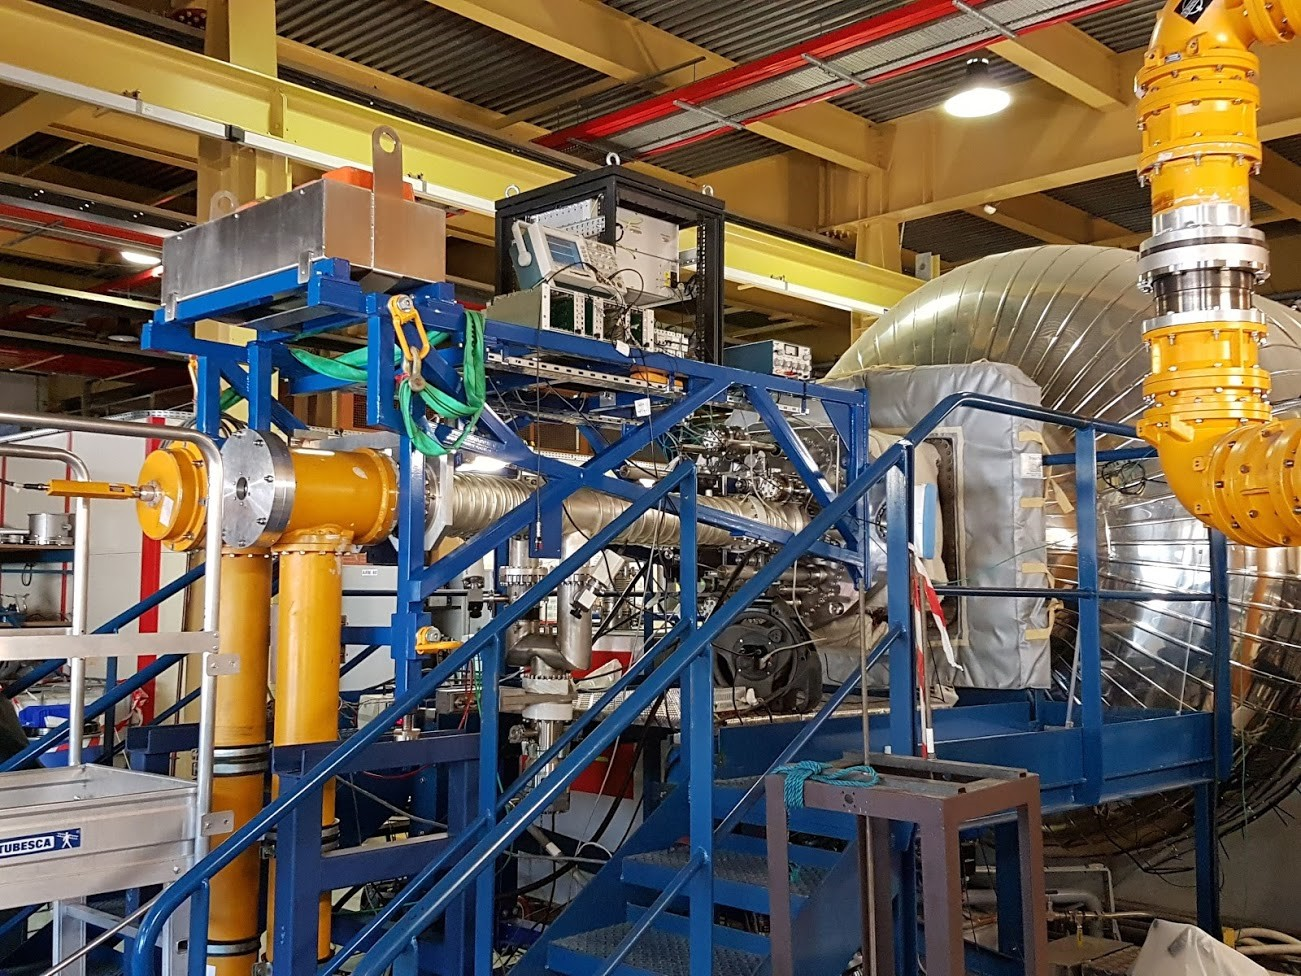
\includegraphics[width=0.95\linewidth]{figures/titan}
	\caption{WEST IRH Antenna IC Q4 installed in the TITAN vacuum chamber. The high power RF input (visible at the right side in yellow) is not yet connected to one antenna side.}
	\label{fig:titan}
\end{figure}


\begin{figure}
	\centering
	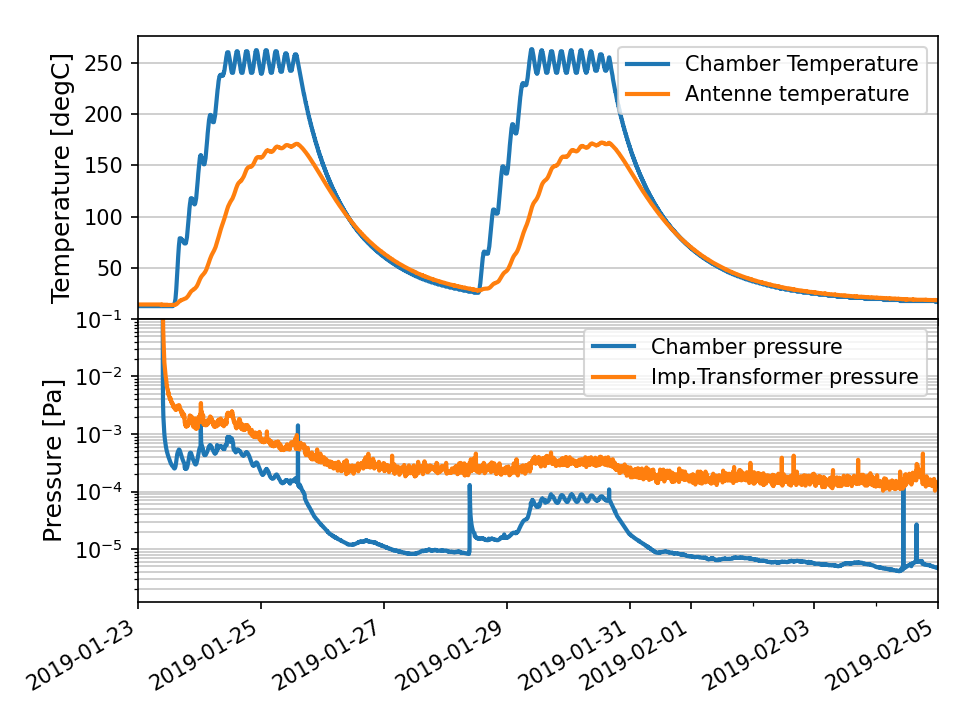
\includegraphics[width=0.95\linewidth]{figures/baking}
	\caption{WEST ICRH Antenna IC Q4 baking and leak tests. Top: chamber and antenna temperatures. Bottom: chamber and impedance transformer pressures.}
	\label{fig:baking}
\end{figure}

\subsection{Fault Detection}
The WEST ICRH system uses a combination of several interlocks to detect faults and RF breakdowns throughout the antennas \cite{hillairet2015-2, helou2020}. In case of fault detection, the two generators feeding an antenna are cut-off within 10 to \SI{50}{\micro\second} then re-applied after 30 to \SI{50}{\milli\second} (depending on the interlock, which in turns can give an idea on the interlock that has triggered). In addition to the standard reflected power ($P_{\mathrm{ref}}/P_{\mathrm{fwd}}$) and Sub-Harmonic Arc Detection (SHAD) systems \cite{berger-by2007}, a new optical arc detection system monitoring the low impedance regions around the T-junctions come in reinforcement. This system relies on 8 optical fibres per antenna associated with fast photodetectors ($<\SI{10}{\micro\second}$) looking at various regions of the low impedance T-junctions. Abnormal events can also be detected from the antenna voltage measurements. Hence, RF power is stopped within \SI{10}{\micro\second} (then reapplied after \SI{30}{\milli\second}) in case of i) voltages lower than \SI{10}{\kilo\volt} when the forward power larger than \SI{100}{\kilo\watt}, meaning RF power does not reach properly the antenna front-face or ii) if a relative difference in voltages between straps is higher than 50\% (unbalance). A  turbomolecular pump connected to at the back of each antenna helps to improve the vacuum level inside both impedance transformers. To prevent sustaining undetected RF plasma discharges which may arise inside these antenna vacuum sections, the RF power is stopped if the pressure measured by vacuum gauges close to the pump is higher than \SI{4.5e-3}{\pascal}, then reapplied when the pressure is below \SI{2.2e-4}{\pascal}.

The RF conditioning after an air venting of the WEST ICRH antennas is performed as follows. Each antenna side is separately energized for \SI{20}{\milli\second} pulses until to reach a stable maximum voltage of \SI{20}{\kilo\volt}. Then, both sides are combined in dipole phasing and forward power then duration are progressively increased. Interestingly, the kind of interlock which triggers, indicated by the marker type and colour scale in figure~\ref{fig:arcdetection}, vary throughout the conditioning process, i.e. the progression of the RF conditioning from low voltages/durations (\SI{5}{\kilo\volt} /\SI{20}{\milli\second}) up to high voltages/durations (\SI{27}{\kilo\volt}/\SI{5}{\second}). While both reflected power and SHAD detectors trigger mostly for high voltage breakdowns (simultaneously or not) \cite{dinca2011}, other kinds of breakdowns often undetected with the two later systems were detected with the new optical arc detectors. These breakdowns generally occur during the beginning of the conditioning phases, but also during plasma operation. Max pressure interlocks trigger in case of severe outgassing, which occurs naturally as the RF energy increases and as long as the antenna RF surfaces are not yet sufficiently conditioned. During plasma operation, all of these interlocks can be triggered, in combination or not. These preliminary results confirm the importance of combining operational safety systems as the location and the breakdown type vary depending on the RF circuit, voltages and material surface properties' evolution \cite{dinca2011-1}. No significant damage has been observed on the antenna front-faces and internal elements since their installation. 

\begin{figure}
	\centering
	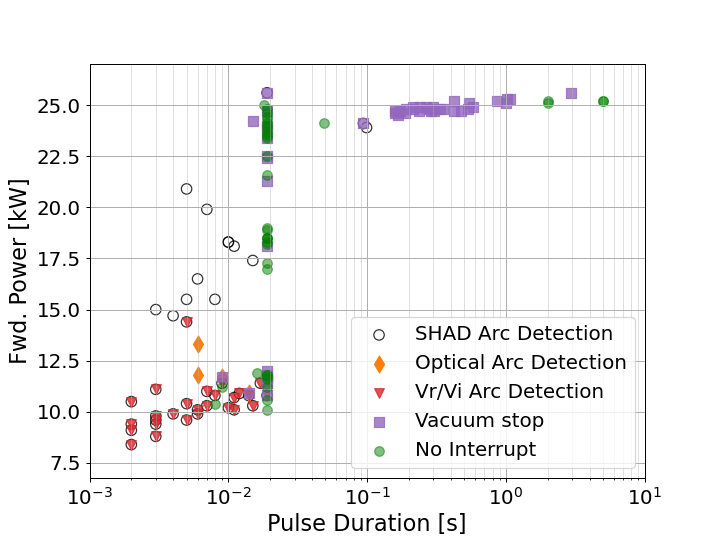
\includegraphics[width=0.95\linewidth]{figures/arc_detection}
	\caption{Example of vacuum conditioning process (from Q1 antenna in 2020), with mean strap voltage as a function of the RF pulse duration. RF conditioning starts at low forward power and duration (\SI{20}{\milli\second}) and the power then the duration are increased until achieving stable pulses (no interruption).}
	\label{fig:arcdetection}
\end{figure}



\section{Plasma Experiments}
\subsection{Key Achievements}
The commissioning phase on WEST plasmas was relatively short, only two days for each antenna were required to reach 1 to \SI{1.5}{\mega\watt}. After this commissioning phase, all three antennas have been operated simultaneously on WEST plasmas. The antennas are operated at a slightly different frequencies (around \SI{150}{\kilo\hertz} shift between antennas) to reduce cross-talks between antennas. A maximum coupled power of \SI{5.8}{\mega\watt} with all three antennas combined has been obtained after around 50 plasma discharges (close to \SI{2}{\mega\watt} per antenna). In combined operation with the Lower Hybrid Current Drive (LHCD) system, a total injected RF power of up to \SI{8}{\mega\watt} has been achieved during few seconds\cite{bucalossi2021}. 

%\begin{figure}
%	\centering
%	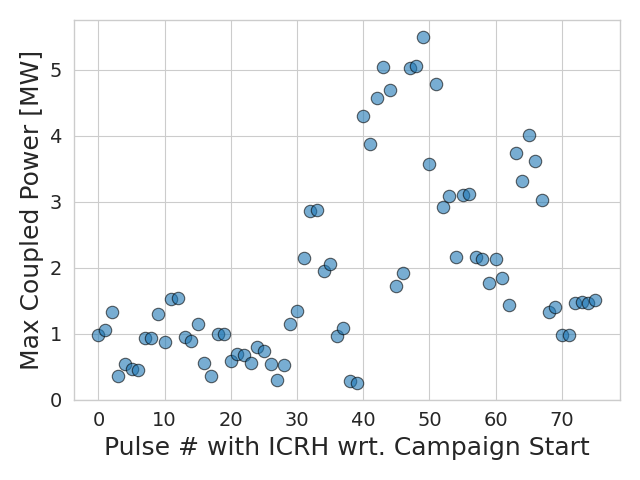
\includegraphics[width=0.95\linewidth]{figures/WEST_ICRH_CoupledPower_vs_pulse}
%	\caption{Evolution of the coupled power for the number of pulses since the start of the 2019 campaign (ICRH–only pulses illustrated). }
%	\label{fig:westicrhcoupledpowervspulse}
%\end{figure}


\subsection{Antenna Load Resilience and Operation}
The intrinsic load tolerance property of the WEST ICRH antennas, already demonstrated during commissioning and first plasma experiments \cite{helou2020}, has been confirmed in the last experimental campaigns. An example of the load resilience of the WEST antennas is illustrated in figure~\ref{fig:westic55589summarypellet} with WEST pulse \# 55589. During this pulse, 5 deuterium pellets have been injected from the high field, leading to fast density increases, correlated with fast changes in the antenna coupling resistance (from 0.5 to \SI{2}{\ohm}).  Figure~\ref{fig:westicrh55589loadresilienceq4} shows the SWR evolution with coupling resistance during the third pellet injection and is compared to the antenna RF model simulation. The red dashed line illustrates the generator SWR limit to couple \SI{3}{\mega\watt} per antenna (\SI{1.5}{\mega\watt} per generator). The gray dashed line represents for reference the SWR that would have been reached if the antenna was not load-resilient (cf.\cite{helou2020} for additional details). 

The operation of the antennas is relatively straightforward, as once the antenna tuning capacitors are properly set up for a given frequency, the antenna load tolerance accepts small capacitance deviations from the ideal match point. Excluding effects on plasma heating efficiency and impurities production, changes in plasma parameters such as minority concentration, fluctuations of the fast wave cut-off layer or minor changes in resonance layer location do therefore not affect the antenna operation significantly. This feature was particularly appreciated during the C4 experimental campaign, as it was still possible to couple RF power to various plasma scenarios despite that few obsolete motor controllers had broken down, prohibiting the movement of some capacitors on two distinct antennas. The motorization system has been fully refurbished for the C5 campaign. 

All antennas are equipped with dedicated gas puffing valves, poloidally distributed 15 to \SI{20}{\centi\meter} behind the antenna lateral limiters, to improve the coupling conditions. However, while the antenna coupling slightly increased at the modest levels of gas flux injected by these valves (\SI{1e21}{el/\second}), the core plasma density was no more controlled due to the limited pumping capabilities of WEST at that time. Improvement of the WEST pumping capabilities for future experimental campaigns gives hope to use local gas puffing as an effective operational tool to improve the ICRH performance, like adopted in other devices such as JET and AUG \cite{jacquet2016, lerche2016}.

\begin{figure}
	\centering
	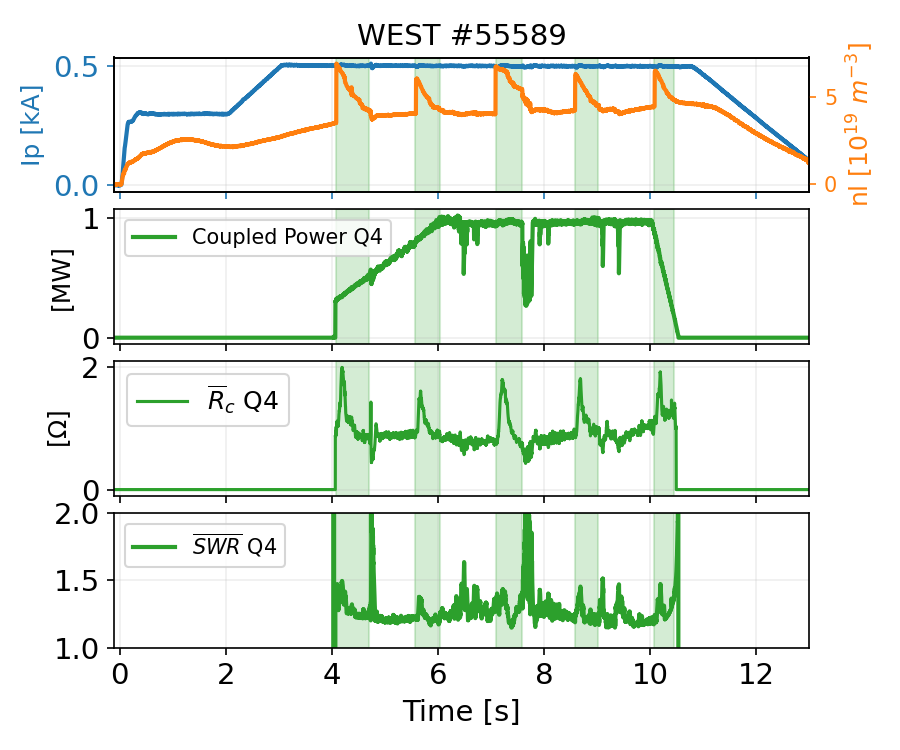
\includegraphics[width=0.95\linewidth]{figures/WEST_IC_55589_summary_pellet}
	\caption{Antenna Load Resilience Demonstration using pellet injections.}
	\label{fig:westic55589summarypellet}
\end{figure}

\begin{figure}
	\centering
	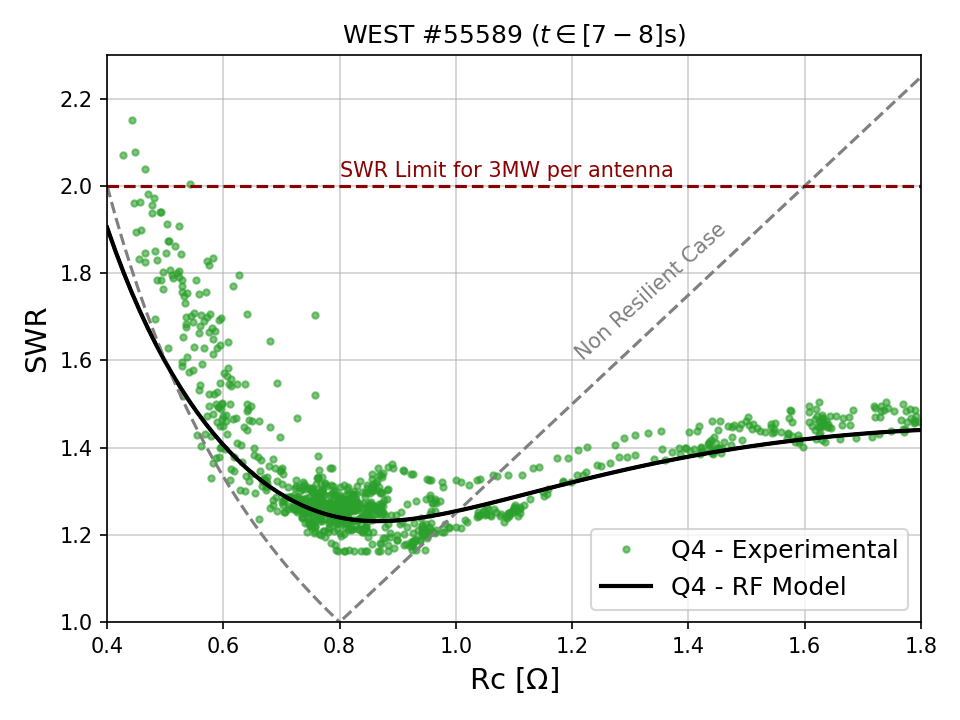
\includegraphics[width=0.95\linewidth]{figures/WEST_ICRH_55589_load_resilience_Q4}
	\caption{Standing Wave Ratio (SWR) versus coupling resistance ($R_c$) for the WEST ICRH antenna Q4 (WEST pulse \#55589) and RF modelling (plain line). The behaviour of a non-resilient antenna is indicated for reference (dashed line). }
	\label{fig:westicrh55589loadresilienceq4}
\end{figure}


\subsection{Automatic Matching}


The use of real-time matching feedback control to optimize the WEST ICRH antenna response during plasma has been successfully demonstrated \cite{helou2020}. The algorithm follows the same principle as the JET ILA \cite{durodie2015} and is described below for convenience. The capacitors are actuated using a negative feedback loop (figure~\ref{fig:icrhmatchingblobkdiagram}) which aims to minimize the difference $\ZTSP – \ZT$, where $\ZT$ is the input impedance at the T-junction (figure~\ref{fig:westicrhblockdiagram}) and $\ZTSP$ the impedance target (SetPoint), which eventually complex-valued. The impedance $\ZT$ depends on both capacitors, ie. $\ZT=\ZT(C_{\mathrm{top}}, C_{\mathrm{bot}})$. It is numerically deduced from power and phase measurements made at the bi-directional couplers located at the rear of the antenna, using a combination of RF measurements and full-wave simulations \cite{helou2020}. Close to the setpoint $\ZTSP=\ZT(\mathbf{C}_{\mathrm{SP}}) = \ZT(C_{\mathrm{top,SP}}, C_{\mathrm{bot,SP}})$, $\ZT$ can be approximated to:

\begin{equation}
	\ZT (\mathbf{C}) = \ZT (\mathbf{C}_{SP} +  \mathbf{\delta C})\approx \ZTSP + \mathbf{g}^T  \mathbf{\delta C}
\end{equation}
where $\mathbf{g}$ is the gradient vector of $\ZT$ at the setpoint. Separating real and imaginary parts and reordering leads to the desired incremental capacitance changes:

\begin{equation}
	\mathbf{\delta C} \approx \mathbf{D}^{-1} (\mathbf{\ZT} - \mathbf{\ZTSP})
\end{equation}
Where the $\mathbf{D}$ is the matrix of partial derivatives around the setpoint and $\mathbf{\ZT}=(\Re(\ZT), \Im(\ZT))$. However, since this matrix cannot be evaluated in real-time, in practice it is approximated with the sign of its elements, evaluated numerically using the antenna RF model, to give the proper descent direction. Depending on the choice of these signs, the operator can choose one of the two matching solutions. The velocities $\mathbf{V}$ at which the capacitors are moved are proportional to the incremental change request $\mathbf{\delta C}$. Figure~\ref{fig:westic55629automatching} illustrates an example of the usage of this method on plasma. As the Radial Outer Gap (ROG) of the plasma decreases, the coupling resistance ($R_c$) increases and the capacitors move apart to improve the antenna matching (SWR decreases).

Because it is based on a RF model linearized close to the match point, the algorithm converges only if the initial guess point is properly chosen, i.e. as long as the gradient estimate corresponds to a negative descent direction. Future work could investigate further improvements such as non-linear converging (faster velocities when far from the set point, slower when closer)\cite{durodie2017} or control methods allowing to increase the range of the starting point. As the capacitors of each antenna side are currently controlled in parallel, future work will consist of taking into account cross-coupling between left and right sides in a self-consistent way and/or minimize voltage unbalance rather than SWR. The possibility to automatically deactivate the real-time control during fast changes of the plasma is envisaged, if it becomes necessary, for example during ELMy phases, using signals from the WEST interferometry system.

\begin{figure}
	\centering
	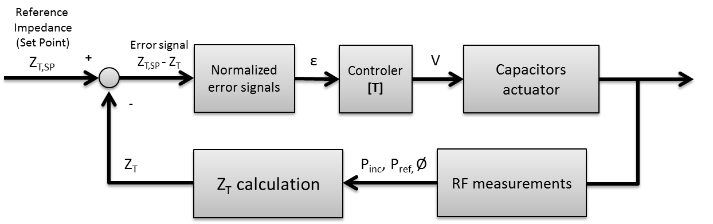
\includegraphics[width=0.95\linewidth]{figures/ICRH_matching_blobk_diagram}
	\caption{Real-Time Matching Algorithm Block Diagram.}
	\label{fig:icrhmatchingblobkdiagram}
\end{figure}

\begin{figure}
	\centering
	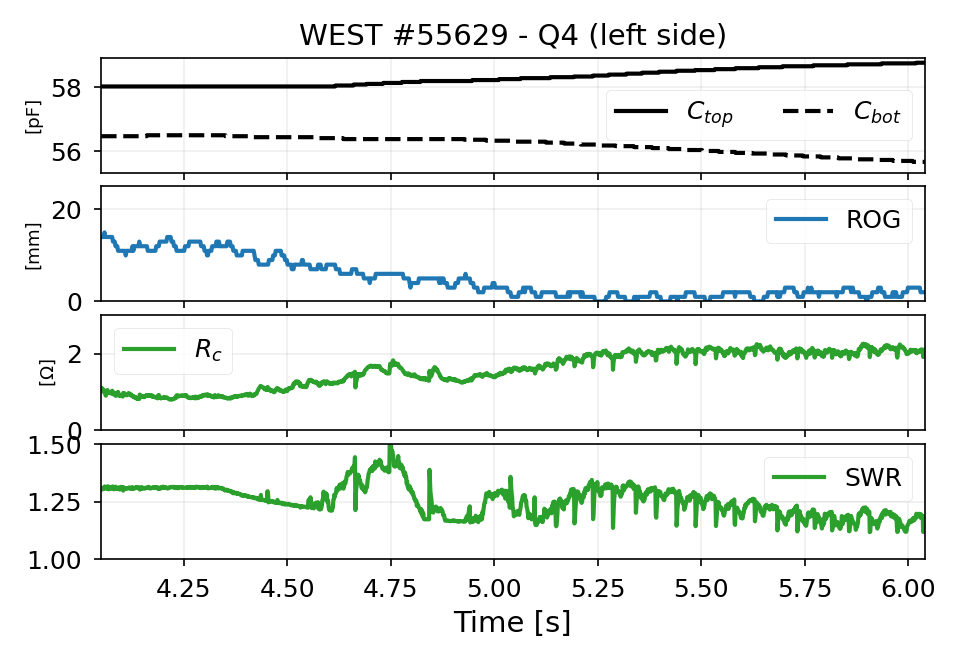
\includegraphics[width=0.95\linewidth]{figures/WEST_IC_55629_auto_matching}
	\caption{Example of real-time matching: As the Radial Outer Gap (ROG) of the plasma decreases, the coupling resistance ($R_c$) increases and the capacitors move to improve the antenna matching (SWR decreases toward 1).}
	\label{fig:westic55629automatching}
\end{figure}


\subsection{Phase Control}

On WEST ICRH antennas, the forward power is generated by two tetrodes\cite{kuus1989}, one for each side of the antenna. The toroidal phase between the left and right sides is achieved by frequency-modulating the right side, the left side being the reference. Initially, the input signal was taken from the toroidal phase between forward powers and the toroidal phase between strap voltages was derived from a linear combination of additional phase measurements. However, this method gave unstable results due to antenna-dependent phase roll-overs occurring in electronic cards. The system has been further improved in the C5 experimental campaign, to measure directly the toroidal phase between (top) strap voltages as the input signal to control. The phase is regulated using an FPGA-based PID whose typical response time to change request is approximatively \SI{50}{\micro\second} and has been found very robust on each antenna to plasma changes. As an example, figure~\ref{fig:westic56469phasecontrol} illustrates the performances of the toroidal phase control for the Q2 antenna on plasma in which the Radial Outer Gap (ROG) is oscillating by $\pm\SI{5}{\milli\meter}$. The phase feedback control has been found very robust to plasma changes. Despite the changes in the coupling resistance, the accuracy of the toroidal phase is in the order of $\pm\SI{2}{\degree}$. The phase error can be increased to $\pm\SI{5}{\degree}$ when multiple antennas are used at the same time or in case of bad absorption, as the phase measurements do not discriminate with frequency and are thus affected by antennas cross-talk and/or multiple passes in the plasma. The role of the antenna toroidal phase in impurity production is discussed in the next section. 

\begin{figure}
	\centering
	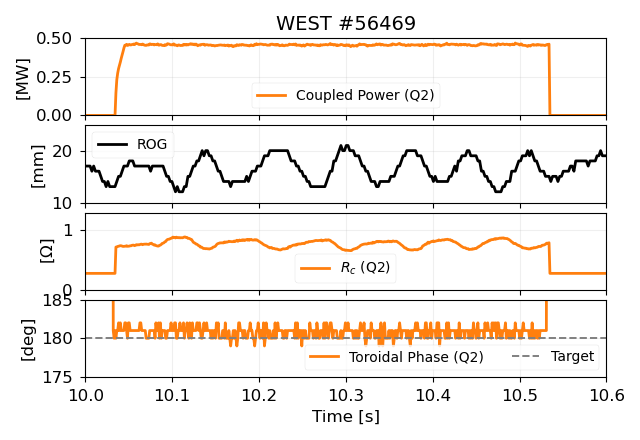
\includegraphics[width=0.95\linewidth]{figures/WEST_IC_56469_Phase_Control}
	\caption{Example of toroidal phase control on an oscillating radial outer gap plasma.}
	\label{fig:westic56469phasecontrol}
\end{figure}

\subsection{Radiated Power and Impurity Production}
When the isotopic ratio $n_H/(n_H+n_D)$ is in the expected range for H minority heating scenarios (i.e. from 5 to 10\%) and the toroidal phase properly tuned to dipole, the radiated power measured in 2019 and 2020 scales with the total power (Ohmic + total RF coupled power) and weak specific effect of LH or ICRH RF power has been found. This is illustrated in figure~\ref{fig:westc4c5pradvsptot} for a large set of plasma scenarios, where each point represents a stable 200 ms time window during which the considered quantity has a relative change below 10\%. High-performance plasma experiments conducted on WEST in 2019 have proven that the ICRH system is a key player in achieving edge density pedestal and H-mode transitions \cite{goniche2021,vermare2021}. Several multiple transitions from L to H modes have been obtained and an H-mode phase of up to \SI{4}{\second} has been sustained with the combination of ICRH and LHCD \cite{bucalossi2021}. However, the sustainment of stable H-modes in WEST is presently impeded by the concomitant increase of core radiation level after a transition. It results in oscillatory edge dynamics also impacting ICRH antennas, decreasing the coupling and eventually the coupled power. Additionally, WEST scenarios are also currently hampered by the issue of burning through the tungsten radiation peak at 1.5-\SI{3}{\kilo\electronvolt}, due to a limited level of central electron heating including when applying ICRH \cite{goniche2021}. Future work will concentrate on optimizing the RF heating scheme to ICRH+LHCD plasma scenarios, especially to increase the central temperature as soon as possible in the discharge. A 3MW/CW ECRH system is also under preparation for WEST\cite{bucalossi2021}. This system will be used in particular for the central heating of the plasma during the very early phase of current ramp up.

The specific role of the ICRF waves in modifying the Scrape-Off Layer has been evidenced using visible spectroscopy and infrared measurements \cite{colas2020, urbanczyk2019, urbanczyk2021}. 17 lines of sight are looking at both lateral limiters of the Q2 antenna (8/9 lines on the left/right limiters respectively). The W-I line (\SI{400.8}{\nano\meter}) brightness is used a proxy of the W gross erosion. When an antenna is powered, the brightness is larger (for a constant total power) than when the antenna is not energized and the amplification factor depends on the antenna voltages. Figure~\ref{fig:westic5522355226} illustrates that a toroidal phase departing from the standard dipole phasing (\SI{180}{\degree}) also led to larger brightness on the antenna side limiters and on the magnetically connected Antenna Protection Limiter (APL) but not elsewhere \cite{urbanczyk2019}. Corrected from the drop of coupled power (due to the antenna unmatching as the phase departs from \SI{180}{\degree}) However, W-I line brightness is not simply related to the W core contamination because of the large prompt redeposition of W and transport in the divertor and SOL. Future work will consist of a deeper characterization of the impurity sources and the effect on plasma core using a combination of experiments measuring low ionisation stages (W II to VIII) and edge transport simulations. At this stage, the operational domain explored so far does not allow us to differentiate the impact of LHCD or ICRH antennas on the core radiation level. New low-Z materials antenna lateral limiters are under design for both LHCD and ICRH antennas. It is expected to install them progressively, allowing direct comparisons between antennas equipped with W or low-Z antenna limiters on WEST plasma.

\begin{figure}
	\centering
	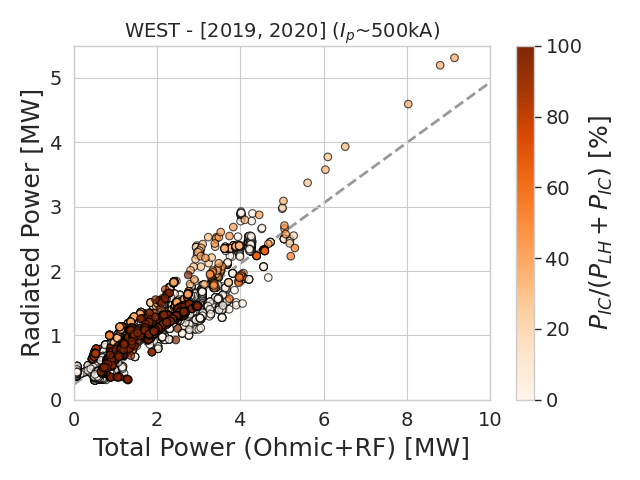
\includegraphics[width=0.95\linewidth]{figures/WEST_C4_C5_Prad_vs_Ptot}
	\caption{Radiated Power versus Total Power during the 2019 and 2020 WEST experimental campaigns. Each point represents a stable 200~ms plateau, independently of the plasma scenario. Plotted data have been filtered for plasma current $I_p$ in [480, 520]~kA  The colour indicates the relative fraction of the ICRH Power in the mix. The dashed line is the best fit linear regression giving $P_{\mathrm{rad}}=0.47 P_{\mathrm{tot}} + 0.23$ with powers in MW.}
	\label{fig:westc4c5pradvsptot}
\end{figure}

\begin{figure}
	\centering
	%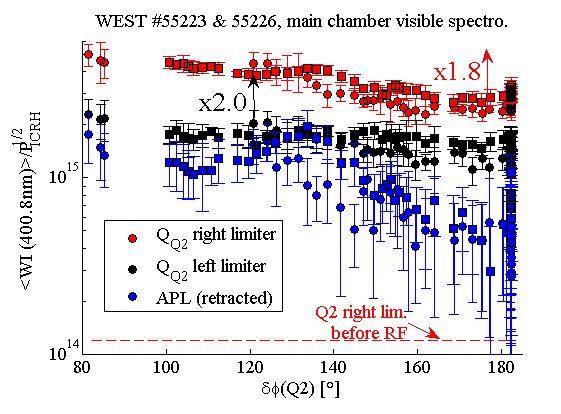
\includegraphics[width=0.95\linewidth]{figures/WEST_IC_55223_55226}
	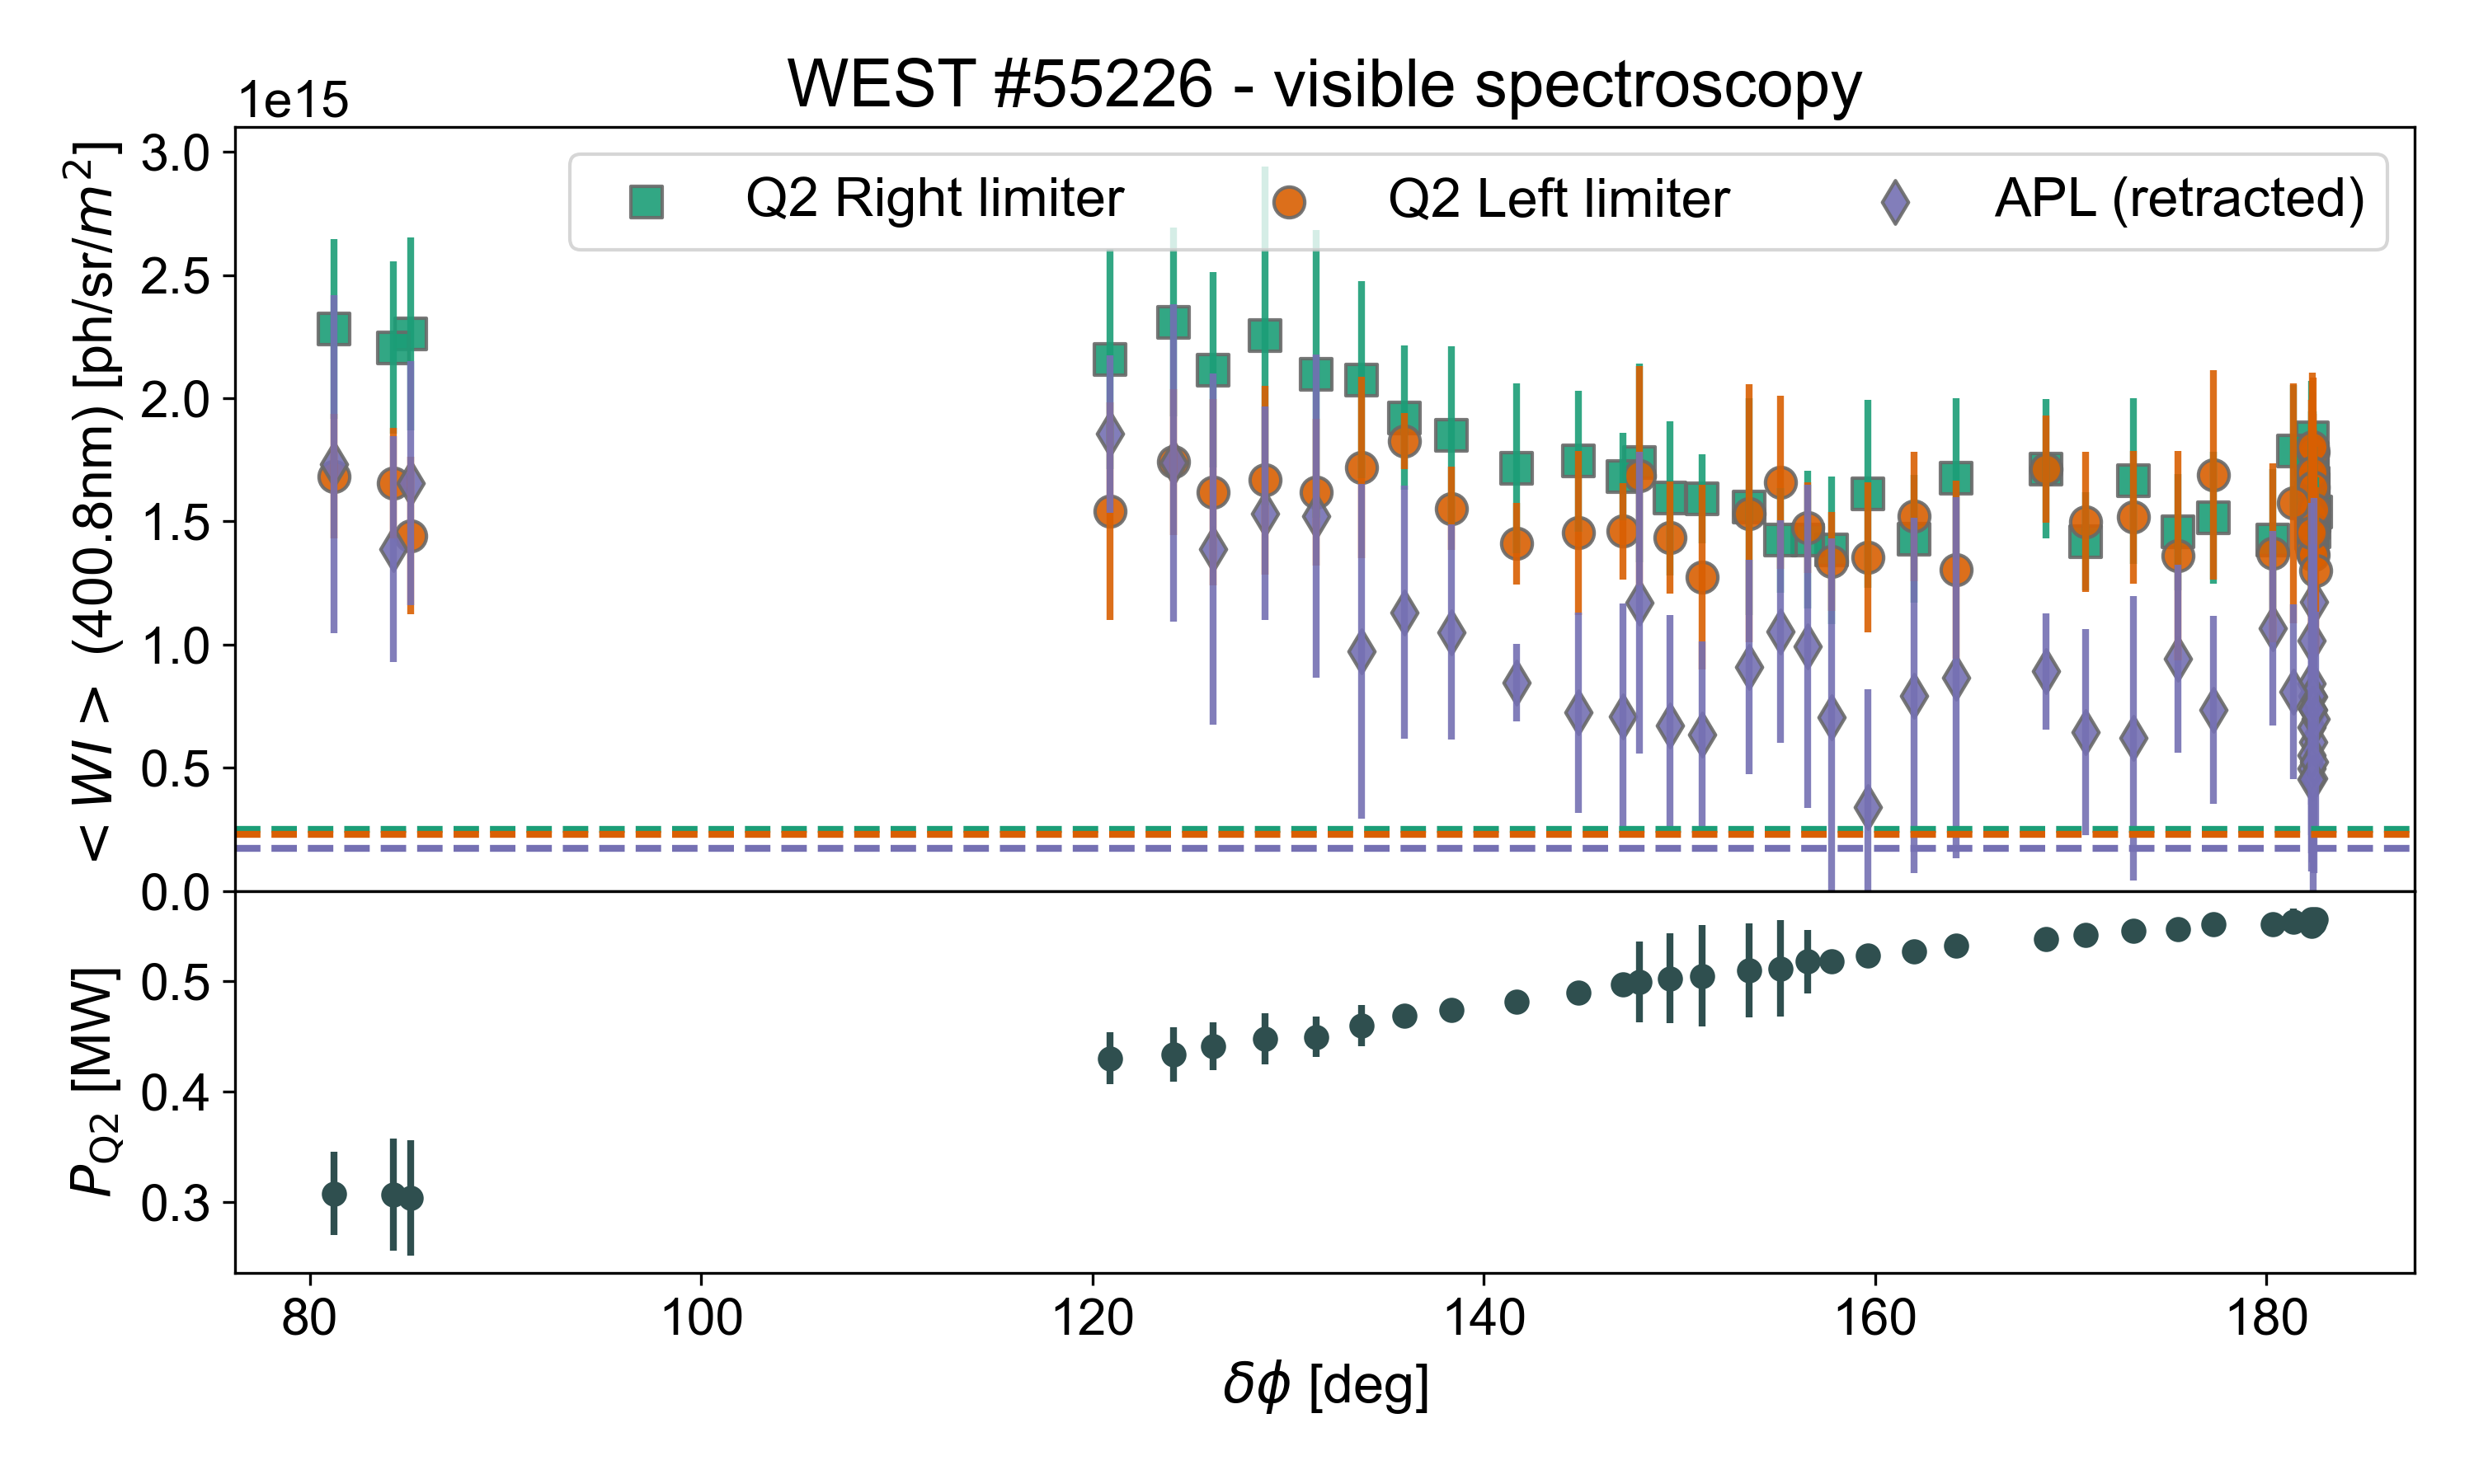
\includegraphics[width=0.95\linewidth]{figures/WEST_IC_55226}
	\caption{Averaged W-I brightness on the Q2 lateral limiters and the Antenna Protection Limiter (APL) during a toroidal phase scan of the Q2 antenna. Dashed lines correspond to the brightness level during the ohmic phase. The evolution of the average coupled power is also illustrated.}
	\label{fig:westic5522355226}
\end{figure}

%\begin{figure}
%	\centering
%	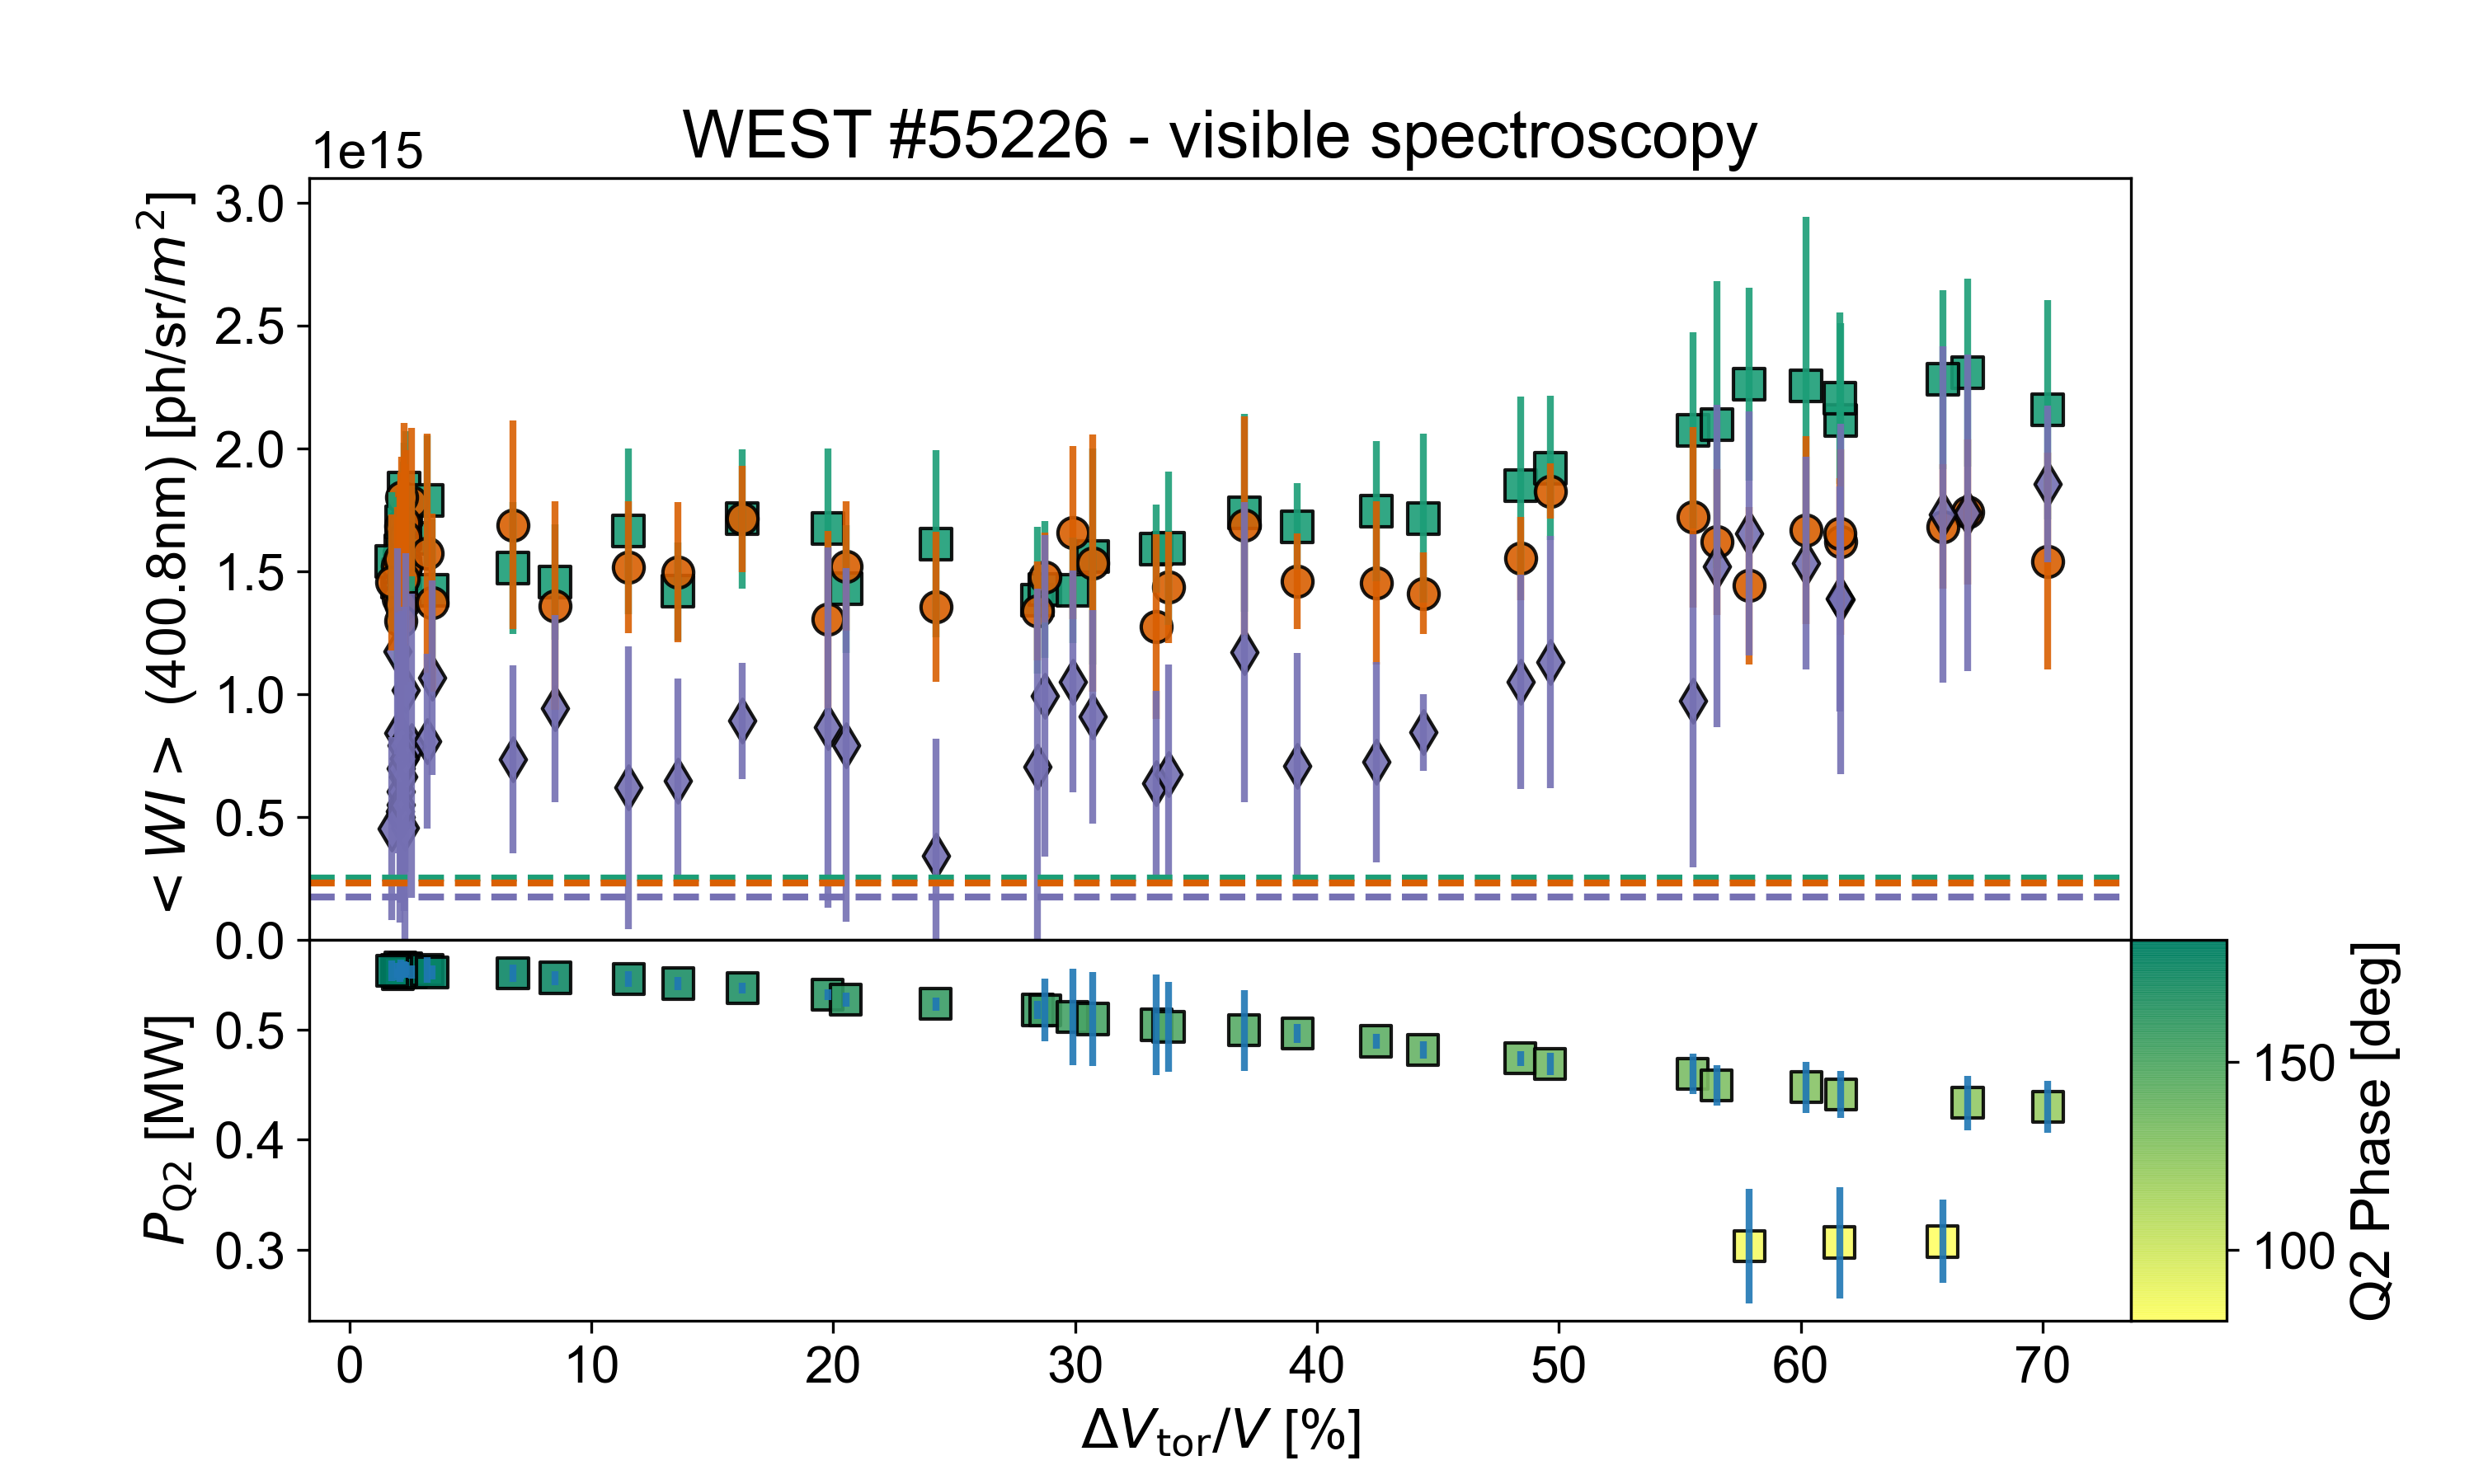
\includegraphics[width=0.95\linewidth]{figures/WEST_IC_55226_vs_unblance}
%	\caption{Averaged W-I brightness on the Q2 lateral limiters and the Antenna Protection Limiter during a toroidal phase scan of the Q2 antenna.}
%	\label{fig:westic5522355226_2}
%\end{figure}


\section{Conclusion and perspectives}
Three identical new WEST ICRH antennas have been designed, assembled then commissioned on plasma from 2013 to 2019, in collaboration with European laboratories and ASIPP within the framework of the Associated Laboratory IRFM-ASIPP. These antennas are load-resilient and compatible with long-pulse operations, a unique combination that no ICRH system before ITER has had to deal with simultaneously. The three antennas have been successfully operated together on plasma in 2019 and 2020. The load resilience capability has been demonstrated and the antenna feedback controls (phase, matching) successfully used. All high confinement mode transitions identified on WEST have been obtained with the combination of LHCD and ICRH systems. Future work will consist of optimizing the combined RF heating scenarios in order to maximize the central temperature and minimize the radiated power.

\section*{Acknowledgements}

This work was carried out under the framework of the Sino-French Fusion Energy centeR (SIFFER, \url{http://www.siffer.science}). This research made use of scikit-rf (\url{http://scikit-rf.org}), an open-source Python package for RF and Microwave applications.



\printbibliography


\end{document}

